\subsection{Choose Alleles}
\begin{figure}[ht]
	\centering
		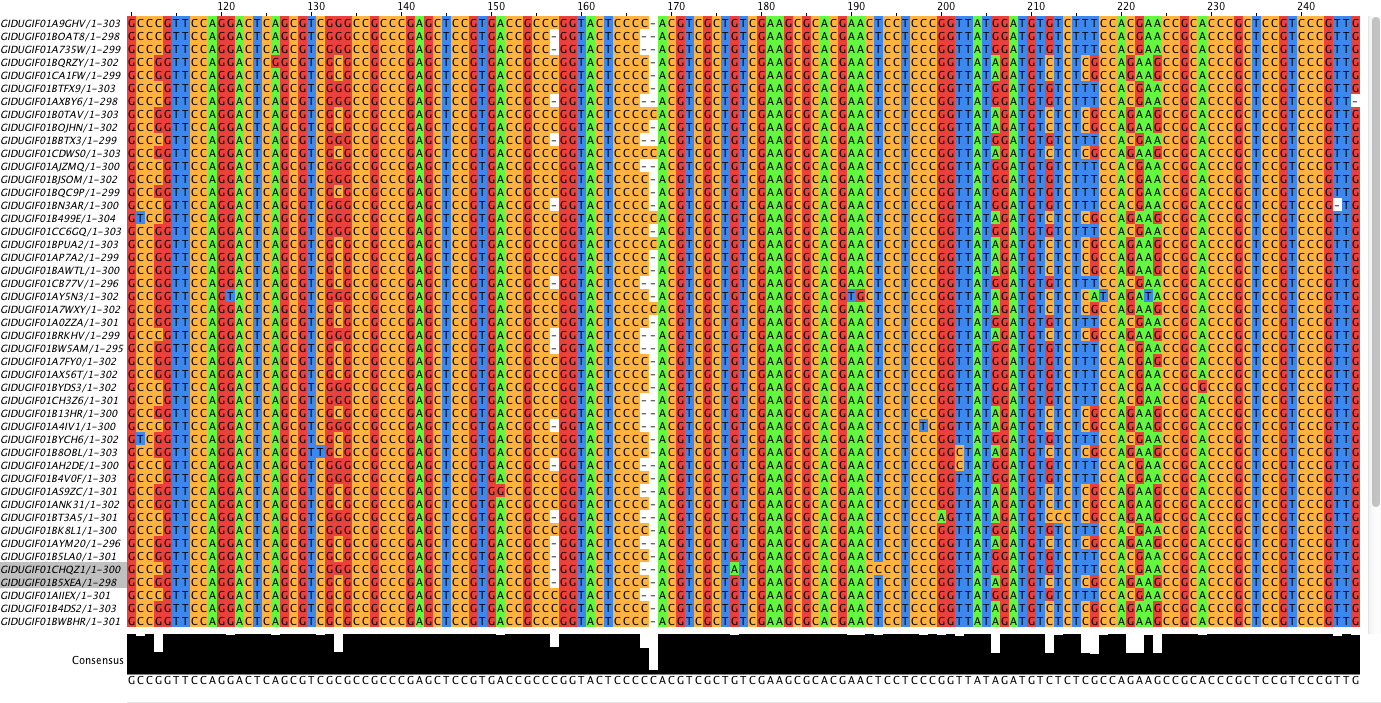
\includegraphics[width=\textwidth]{../pictures/align_example.png}
	\caption{Aligned sequences}
	\label{fig:many_aligned_sequences}
\end{figure}

% Refer to figures

We can think of the alignment like in picture \ref{fig:many_aligned_sequences}, that all sequences are put on top of each other like rows in a matrix, then each column in the matrix represents a position in the sequence. The differences between two alleles are of course the differences in certain positions of the sequence, the rest will be identical. But as we can see, there are some noice in the form of read errors that needs to be distinguished from true variation. Most of these columns will have more or less the same nucleotide in all rows but in some cases there will be a distribution between two or more bases, in the \emph{true} sequences we do not allow more than two variants in one position since this would imply more than two alleles. If there is enough variation in a position for us to believe that is true and not an error we call this position a \emph{variable position}.\\

If there is no variable positions among the sequences the individual is a \emph{homozygote}, if there are at least one variable position the individual is a \emph{heterozygote}. The problem here is to determine if a variation is real or created during sequencing. 

\subsubsection{1. Count the frequencies for each position}


For each position of the exon, which is represented by a column in our aligned matrix, we look at the distribution over the nucleotides or insertions. The original sequence is 270 base pairs long, but as a consequence of insertions and deletions the length might vary. We call the positions $n$ and the frequencies $q_a$ where $a\in \{A,C,G,T,-\}$. So each position $n$ has a distribution like $d_n: \lbrack q_A=x_1, q_C=x_2, q_G=x_3, q_T=x_4, q_{-}=x_5 \rbrack $ and $\sum_{i=1}^{5}x_i = 1$.\\
We call the frequency of the most abundant variation in position $n \, q_n^1$, the second most abundant $q_n^2$ and so on, these frequencies represents a nucleotide. Then if $q_n^2 = 0 \implies q_n^1=1$, and both alleles have the same nucleotides in position $n$, and if $q_n^1 = 1, \, \forall \, n \implies$ homozygous individual.

\subsubsection{2. Choose a treshold for variable positions.}

We have to decide \emph{when} we say that a position is variable since this will determine if an individual is hetero- or homozygote and for which positions the sequences differs. If $q_n^2$ is very small we might assume that the distribution is a consequence of some kind of error in the process. We want to find a treshold that is reasonable, if we for example set the threshold such that if the second most abundant nucleotide is in 10\% of the reads we call it a variable position(implying a heterozygote), this will mean that an individual with 20 reads needs the same variation in only 2 of them to give rise to a second allele, this might be accomplished by read errors so we need to be a bit careful. In the figure \ref{fig:het_hom_relation} we can see how the relation between hetero- and homozygote individuals varies when changing this treshold for $q_n^2$.

\begin{figure}[ht]
	\centering
		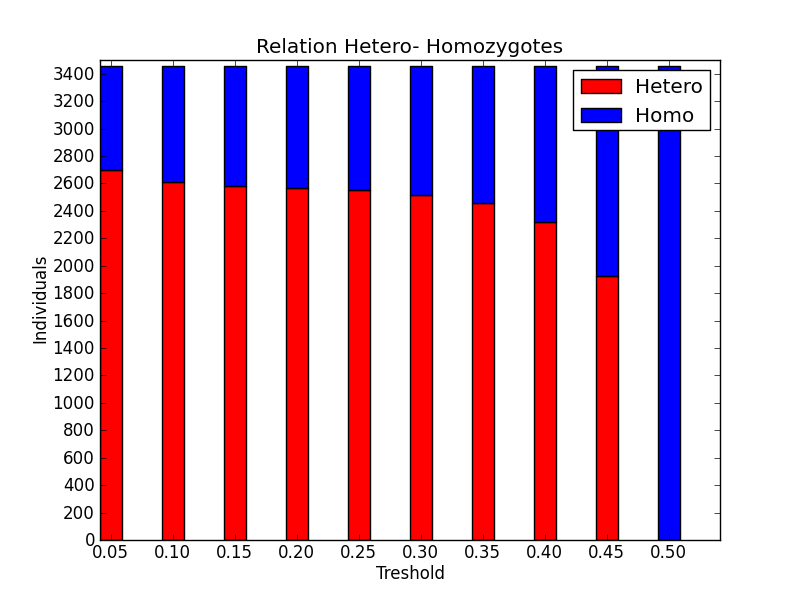
\includegraphics[width=0.6\textwidth]{../pictures/het_hom.png}
	\caption{Relation between hetero and homozygotes when $q_n^2 < treshold$. It is enough with a single variable position to count the individual as a heterozygote.}
	\label{fig:het_hom_relation}
\end{figure}


There are many errors in our data and we need to be careful of creating novel sequences with these errors. We prefer to miss some alleles (e.g. say that an individual is homozygote when they are heterozygote) in a few individuals rather than to report false sequences. We chose the Variable Position Treshold ($VPT$) such that the second most abundant nucleotide must be present in at least 35\% of the reads to qualify as a variable position.\\

\subsubsection{3. Build the alleles}

To produce the alleles we walk through the sequence, starting from position 1 and look at $q_1^2$. If $q_n^2 \leq \, VPT$ we add the nucleotide represented by $q_n^1$ to position $n$ in both allele sequences $A^1$ and $A^2$. If $q_n^2 > \, VPT$ we have a variable position, $V_i$, so one variant should be added to both alleles at position $n$, we denote this as $A^1_n$ and $A^2_n$. If it is the first variable position, $V_1$ (notice that this is not the first position of the sequence, it is the first variable position for the sequences), it does not matter how we add the variant since both alleles are identical up till now. If the n:th position is a variable position $V_i, \, i \neq 1 $ we need to decide which variant should be added to which allele. One thing that makes the situation complicated is the chimeric formations of the sequences, remember that they consist of segments of sequences that has been copied and annealed together to form new artificial sequences. Our method is based on the idea that the majority of the reads of an individual have the correct sequence if looked at in portions.\\
So when we have a variable position $n = V_i, \, i \neq 1$, that is position $n$ which is also the variable position number $i$, we sort all sequences based on what variation they had in the previous variable position, $V_{i-1}$, into two groups $G^1$ and $G^2$. Each of these groups have a consensus nucleotide at every position $n$ that we call $G^j_n$. Since we sorted the sequences based on what nucleotide they had in position $V_{i-1}$ we know that $G^1_{V_{i-1}} \neq G^2_{V_{i-1}}$. We then compare $G^1_{V_{i-1}}$ to $A^1_{V_{i-1}}$ if they are the same we set the consenseus nucleotide $G^1_n$ to $A^1_n$ and $G^2_n$ to $A^2_n$. If $G^1_{V_{i-1}} \neq A^1_{V_{i-1}}$ we set $G^2_n$ to $A^1_n$ and $G^1_n$ to $A^2_n$.

\subsubsection{4. Produce the final allelic sequences}

There are now two alleles with almost identical sequences if the individual is heterozygote or two identical alleles if homozygote. Some problems are still left; there are positions where $q_n^1$ represents $-$, which means that the alleles have a deletion in position n, these has to be filled with something. To do this we want to find the most similar reference sequence and insert the corresponding variant here. The idea here is that all sequences have a relationship in the sense that they have evolved from the same original sequence. So the sequence that is most similar over the full length is most likely to have the same base in the unknown position in question. This is done by calculating the similarity between the allele and all of the reference sequences and then fill the gaps with the corresponding nucleotide from the most similar reference sequence.

\subsubsection{5. Remove the tags.}
We assume that our algorithm made a perfect alignment so we can simply cut the beginning and end of each sequence to get the full exon only.
